\part*{Ejercicio 8}

\subsection*{Trigger HC-SR04}

El primer paso en el diseño del circuito fue implementar un bloque circuital que proporcione el pulso de trigger al sensor HC-SR04, el cuál, como indica en las especificaciones, debe ser de $10 \mu seg$, sin embargo, habiéndose realizado pruebas utilizando una placa de experimentación Arduino UNO, se determinó que se puede disparar el sensor con pulsos de ordenes superiores de extensión. Esta observación tiene relevancia, ya que generar un pulso tan breve mediante un pulsador mecánico trae ciertas complejidades. Dicho esto, a continuación se explica el circuito utilizado para generar el pulso.
\bigskip

\begin{figure}[H]
\begin{center}
\begin{circuitikz}[scale=1] \draw
(0,0) node[ground] {}
	to[push button = Push Button] (0,2.5)
	to[R = 10k, *-*] (0,5)
	to (0,5.5) node[vcc]{Vcc}
	(0,5) -- (2,5)
	to[R=3k3, -*] (2,2.5)
	to[C=0.01$\mu$F](0,2.5)
	(2,2.5) -- (3,2.5)
	(3.5,2.5) node[invschmitt]{}
	(4,2.5) to[short,-o] (4.5,2.5)
	node[right]{$V_{out}$}
;
\end{circuitikz}
\end{center}
\caption{Circuito para generar pulso de $30 mseg$} \label{8_fig1}
\end{figure}

Los valores del capacitor de $0.01\mu F$ y la resistencia de $3k3$ se determinaron al resolver el transitorio del circuito, y considerando los valores $V_{T_{MAX}}^+$(Máximo valor en la entrada para el cuál tengo HIGH en la salida del inversor Scmhitt trigger 74HC14) y el valor de $Vcc$ para obtener un pulso de aproximadamente $30 \mu seg$. La respuesta teórica aproximada que se obtiene en la entrada y la salida del inversor que se muestra en la Figura \ref{8_fig1} se muestra en la Figura \ref{8_fig2}.

\begin{figure}[H]
\centering
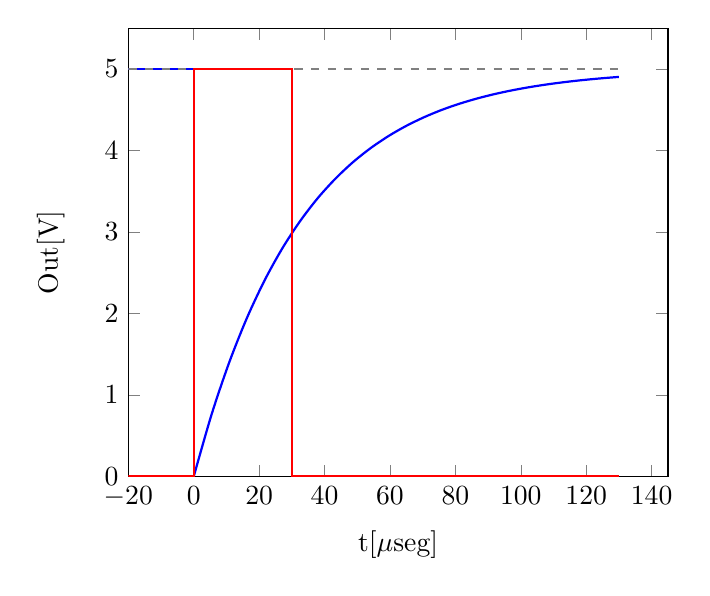
\begin{tikzpicture}
 \begin{axis}[
   scaled ticks=false,
   xmin=-20,
   ymin=0,
    x label style={at={(axis description cs:0.5,-0.1)},anchor=north},
    y label style={at={(axis description cs:-0.1,.5)},rotate=0,anchor=south},
    xlabel={t[$\mu$seg]},
    ylabel={Out[V]}
   ]
    \addplot[domain=0:130, blue, thick,smooth] {5*(1-e^(-x/33))};
    \addplot[domain=-20:100, const plot, blue, no marks, thick] coordinates {(-20,5) (0,5) (0,0)};
    \addplot[domain=-20:130, gray, dashed] {5};
    \addplot[domain=-20:100, const plot, red, no marks, thick] coordinates {(-20,0) (0,0) (0,5) (30,5) (30,0) (130,0)};
\end{axis}
\end{tikzpicture}

\caption{Respuesta del transitorio y la compuerta inversora} 
\label{8_fig2}
\end{figure}

Por supuesto no debe enviarse la 'instrucción' de triggerear el HC-SR04 si el circuito no habilita a hacerlo, es decir, si el circuito esta procesando una medición anterior. Para esto, se utiliza una compuerta AND con una entrada linkeada al registro que va a determinar si el circuito esta ocupado o listo para usarse y otra al pulso generado, explicado anteriormente. La lógica que determine si el circuito está o no ocupado se explicará mas adelante.


\begin{figure}[H]
\centering
\begin{center}
\begin{circuitikz}[scale=1] \draw
(0,0) node[ground] {}
	to[push button = Push Button] (0,2.5)
	to[R = 10k, *-*] (0,5)
	to (0,5.5) node[vcc]{Vcc}
	(0,5) -- (2,5)
	to[R=3k3, -*] (2,2.5)
	to[C=0.01$\mu$F](0,2.5)
	(2,2.5) -- (3,2.5)
	(3.5,2.5) node[invschmitt]{}
	(4,2.5) to[short] (4.5,2.5)
	(6.5,1) node[and port](myand1){}
	(4.5,2.5) -| (myand1.in 1)
	(4.5,0) -| (myand1.in 2)
	(4.5,0) node[left]{CAN\_TRIGGER}
	(myand1.out) to[short, -o] (7,1)
	(7,1) node[right]{HC-SR04 TRIGGER}
;
\end{circuitikz}
\end{center}
\caption{Circuito para triggerear HC-SR04}
\label{8_fig3}
\end{figure}

La variable CAN TRIGGER determina si se puede o no triggerear el sensor. Esta variable es función de dos variables, una es CIRCUIT READY e indica si el circuito está listo para utilizarse y la otra es TRIGGER\_ENABLE, y habilita o deshabilita el trigger manualmente. El diagrama lógico que las vincula se muestra en la Figura \ref{8_fig6}:

\begin{figure}[H]
\centering
\begin{circuitikz}
\draw
(0,0) node[and port](myand){}
(myand.in 1)++(left:1.5) node(trg_en){}
(myand.in 2)++(left:1.5) node(c_ready){}
(trg_en) node[left](){TRIGGER\_ENABLE}
(c_ready) node[left](){READY}
(trg_en) to[short,o-] (myand.in 1)
(c_ready) to[short,o-] (myand.in 2)
(myand.out) to[short,-o] ++(right:1)
node[right](){CAN\_TRIGGER}
;
\end{circuitikz}
\caption{Logica a la entrada del contador} \label{8_fig5}
\end{figure}


\subsection*{Diseño del Clock}
Uno de los parámetros mas importantes en el diseño del circuito es elegir una apropiada frecuencia de clock, ya que esta nos va a determinar la medición máxima y mínima que nuestro circuito será capaz de realizar. Debido a que contamos con un contador de 8 bits, el numero máximo de 'clicks' que podremos contar está dado por $n_{max} = 2^8-1=255$.
El fabricante del sensor HC-SR04 nos indinca que el \emph{echo} generado, el cual nos indica la distancia medida por el sensor, está dado por:

\[\frac{\mu seg}{58} = cm \]

Si definimos:


\[
  \begin{cases}
    d:\text{distancia medida en cm }\\
    n:\text{'ticks' de reloj contados}\\
    T_{\mu}:\text{Período del clock en $\mu$seg}
  \end{cases}
\]

Entonces podemos detrminar los parametros a partir de la siguiente expresión:

\[ \frac{nT_{\mu}}{58}=d\]

Se determinó como condición la distancia mínima a medir, la cual según el fabricante del sensor, es 2cm, y de esta forma se obtuvo que el período del clock \emph{T} debe ser de $116 \mu seg$. La distancia máxima que se podrá medir será de 255 cm. La frecuencia del clock será entonces $f \approx 8.6kHz$.


Para la implementación del clock se decidió utilizar un integrado 555 en modo astable. La configuración del mismo en el modo mencionado se muestra en la Figura \ref{8_fig4}. Las expresión, según la hoja de datos de los integrados 555, para determinar el comportamiento del dispositivo en función de los componentes $R_1$, $R_2$ y $C$ son:

\[
\begin{cases}
	t_H=ln(2)(R_1 + R_2)C\\
	t_L=ln(2)R_2C\\
	T=t_L + t_H	
\end{cases}
\]

Trabajando con estas expresiones, se calcularon los valores de los componentes de forma que se obtenga un clock con los parámetros anteriormente mencionados, y se determinaron:

\[
\begin{cases}
	R_1=3.35 k\Omega\\
	R_2=6.694 k\Omega\\
	C=0.01\mu F	
\end{cases}
\]

\begin{figure}[H]
\begin{center}
\begin{circuitikz}[scale=1]
\draw(-1.5,-2) rectangle (1.5,2); %IC rectangle
\draw (0,0.5) node [align=center]{\large xx-555\\TIMER}; % IC LABEL
% Draw the pins

\draw (0.9,-2) node [above]{GND} -- +(0,-0.5) node [anchor=-45]{1} coordinate (GND); % Pin 1 GND
\draw (-1.5,-1.5) node [right]{TRG} -- +(-0.5,0) node [anchor=-135]{2} coordinate (TRG); % Pin 2 TRG
\draw (1.5,0) node [left]{OUT} -- +(0.5,0) node [anchor=-45]{3} coordinate (OUT); % Pin 3 OUT  
\draw (0.9,2) node [below]{RESET} -- +(0,0.5) node [anchor=45]{4} coordinate (RESET); % Pin 4 RESET
\draw (0,-2) node [above]{CTRL} -- +(0,-0.5) node [anchor=-45]{5} coordinate (CTRL); % Pin 5 CTRL
\draw (-1.5,-.5) node [right]{THR} -- +(-0.5,0) node [anchor=-135]{6} coordinate (THR); % Pin 6 THR
\draw (-1.5,1.5) node [right]{DIS} -- +(-0.5,0) node [anchor=-135]{7} coordinate (DIS); % Pin 7 DIS
\draw (0,2) node [below]{$\mathsf{V_{CC}}$} -- +(0,0.5) node [anchor=45]{8} coordinate (VCC); % Pin 8 VCC

% Start conecting 
\draw(-4,3.5) % Start point
    node [anchor=east]{$V_{CC}$}
    to [short, o-] ++(1,0) coordinate (NOD1) % Use auxiliar coordinate (NOD1)
    to [R=$R_1$,*-*] (DIS -| NOD1) node(NOD3){}% to the point in the intersection between NOD1 and 1 DIS
    to [R=$R_2$,*-*] (THR -| NOD1) node(NOD2){}% idem
    to [short, *-*] (TRG -| NOD1)
    to [C=C,*-*] (-3,-5)
    to [short,*-o] ++(-1,0) coordinate (GND2)
    node [anchor=east]{GND};
    
    %Conect U-1
\draw (VCC) to [short, -*] (VCC |- NOD1);
\draw (RESET) to [short, -*] (RESET |- NOD1);
\draw (TRG) to [short, -*] (TRG -| NOD1);
\draw (CTRL) to [C,l_=0.01nF, -*] (CTRL |- GND2);
\draw (GND) to [short, -*] (GND |- GND2);
\draw (GND2) to [short] (GND2-|GND);
\draw (NOD2) to [short] (THR);
\draw (NOD3) to[short] (DIS);
\draw (NOD1) to[short] (NOD1-|RESET);
\draw (OUT) to[short,-o] ++(right:1) node[right]{Clk \texttiming{LHLHL}};
\end{circuitikz}
\caption{xx555 configurado en modo astable} \label{8_fig4}
\end{center}
\end{figure}

\subsection*{Implementacion del contador}

El integrado elegido para contar la extensión del puslo \emph{ECHO} del sensor HC-SR04 fue un \emph{74HC4040}, el cuál cuenta con 3 modos de funcionamiento, en función de los estados de sus tres entradas $CP$, $CLR$ y , los mismos se detallan en la siguiente tabla:

\begin{center}
\begin{tabular}{c|c|c}
CP & MR & MODO \\ 
\hline 
\texttiming[timing/c/rising arrows, timing/c/arrow pos=.7]{2{C}} & LOW & Hold \\ 
\texttiming[timing/c/falling arrows, timing/c/arrow pos=.7]{HC} & LOW & Count \\ 
X & HIGH & Reset \\ 
\end{tabular} 
\end{center}

Se pretende que en tanto el sensor devuelva un ECHO, el contador este activo, y mientras el sensor no devuelva ECHO, el contador no cuente. Dicho esto, la entrada CP será función del Clk y del pulso ECHO, como se muestra en la Figura \ref{8_fig6}

\begin{figure}[H]
\centering
\begin{circuitikz}
\draw
(0,0) node[and port](myand){}
(myand.in 1)++(left:1.5) node(Clk){}
(myand.in 2)++(left:1.5) node(ECHO){}
(Clk) node[left](){Clk}
(ECHO) node[left](){ECHO}
(Clk) to[short,o-] (myand.in 1)
(ECHO) to[short,o-] (myand.in 2)
(myand.out) to[short,-o] ++(right:1)
node[right](){To CP}
;
\end{circuitikz}
\caption{Logica a la entrada del contador} \label{8_fig6}
\end{figure}

La entrada MR es controlada por un pulsador físico, de forma que esta ponga todas las salidas del contador en LOW, y prepare el circuito para una eventual nueva medición.

\subsection*{Reset Button}

El usuario al pulsar el boton de reset, además de resetear el contador, toggleará un Flip-Flop que almacenará el estado de la variable CIRCUIT READY, ilustrada en la Figura \ref{8_fig3}, para dejar el circuito habilitado para una nueva solicitud de medición.